
%
\documentclass[conference]{IEEEtran}
% Add the compsoc option for Computer Society conferences.
%
% If IEEEtran.cls has not been installed into the LaTeX system files,
% manually specify the path to it like:
% \documentclass[conference]{../sty/IEEEtran}

% \usepackage{epsfig}
% \usepackage{graphicx}
\usepackage{color}
\newcommand{\dean}[1]{\textsf{\emph{\textbf{\textcolor{red}{#1}}}}} 
\newcommand{\red}{\textcolor{red}}
\newcommand{\parham}[1]{\textsf{\emph{\textbf{\textcolor{blue}{#1}}}}} 
\newcommand{\cyan}{\textcolor{cyan}}


\ifCLASSINFOpdf
  \usepackage[pdftex]{graphicx}
  % declare the path(s) where your graphic files are
  \graphicspath{{./figures/pdf/}{../jpeg/}}
  % and their extensions so you won't have to specify these with
  % every instance of \includegraphics
  \DeclareGraphicsExtensions{.pdf,.jpeg,.png}
\else
  % or other class option (dvipsone, dvipdf, if not using dvips). graphicx
  % will default to the driver specified in the system graphics.cfg if no
  % driver is specified.
  \usepackage[dvips]{graphicx}
  % declare the path(s) where your graphic files are
  % \graphicspath{{../eps/}}
  % and their extensions so you won't have to specify these with
  % every instance of \includegraphics
  \DeclareGraphicsExtensions{.eps}
\fi

\usepackage[cmex10]{amsmath}

\usepackage[tight,footnotesize]{subfigure}

% correct bad hyphenation here
\hyphenation{op-tical net-works semi-conduc-tor}


\begin{document}
%
% paper title
% can use linebreaks \\ within to get better formatting as desired
\title{Model-Based Estimation of Intracortical Spatial Properties}


\author{\IEEEauthorblockN{\dean{Dean R. Freestone}\IEEEauthorrefmark{1},
\parham{Parham Aram}\IEEEauthorrefmark{2},
Kenneth Scerri\IEEEauthorrefmark{3},
Michael Dewar \IEEEauthorrefmark{4}, \\
Visakan Kadirkamanathan\IEEEauthorrefmark{2} and 
David B. Grayden\IEEEauthorrefmark{1}}
\IEEEauthorblockA{\IEEEauthorrefmark{1}Department of Electrical and Electronic Engineering\\
The University of Melbourne,
Parkville, VIC, Australia\\ Email: see http://www.neuroeng.unimelb.edu.au/}
\IEEEauthorblockA{\IEEEauthorrefmark{2}Department of Automatic Control and Systems Engineering, University of Sheffield, Sheffield, UK}
\IEEEauthorblockA{\IEEEauthorrefmark{3}Department of Systems and Control Engineering, University of Malta, Msida, MSD, Malta}
\IEEEauthorblockA{\IEEEauthorrefmark{4}Department of Applied Physics and Applied Mathematics, Columbia University, New York, NY, USA}}

% make the title area
\maketitle

\begin{abstract}
%\boldmath

\end{abstract}

\IEEEpeerreviewmaketitle


\section{Introduction}
% no \IEEEPARstart
Discuss model-based estimation


\section{Method}


\subsection{Stochastic Neural Field Model}
The model relates the average number of action potentials $g(\mathbf{r},t)$ arriving at time $t$ and position $\mathbf{r}$ to the local post-synaptic membrane voltage $v(\mathbf{r},t)$. The post-synaptic potentials generated at a neuronal population at location $\mathbf{r}$ by action potentials arriving from all other connected populations is described by 
\begin{equation}
	\label{SpikesToPotential} v\left( {\mathbf{r},t} \right) = \int_{ - \infty }^t {h\left( {t - t'} \right)g\left( {\mathbf{r},t'} \right) \, dt'}. 
\end{equation}
The post-synaptic response kernel $h(t)$ is described by 
\begin{equation}
	\label{SynapticRespKernel} h(t) = \eta(t)\exp{\left(-\zeta t\right)}, 
\end{equation}
where $\zeta=\tau^{-1}$, $\tau$ is the synaptic time constant and $\eta(t)$ is the Heaviside step function. Non-local interactions between cortical populations at positions $\mathbf{r}$ and $\mathbf{r}'$ are described by 
\begin{equation}
	\label{eq:RateBasedInteractions} g\left( \mathbf{r},t \right) = \int_\Omega {w\left( \mathbf{r},\mathbf{r}' \right)f\left( v\left( \mathbf{r}',t \right) \right)\, d\mathbf{r}'}, 
\end{equation}
where $f(\cdot)$ is the firing rate function, $w(\cdot)$ is the spatial connectivity kernel and $\Omega$ is the spatial domain representing a cortical sheet or surface. The firing rate of the presynaptic neurons is related to the post-synaptic membrane potential by the sigmoidal activation function 
\begin{equation}
	\label{ActivationFunction} f\left( v\left( \mathbf{r}', t \right) \right) = \frac{1}{1 + \exp \left( \varsigma \left( v_0 - v\left(\mathbf{r}',t\right) \right) \right)}. 
\end{equation}
The parameter $v_0$ describes the firing threshold of the neural populations and $\varsigma$ governs the slope of the sigmoid. By substituting equation~\ref{eq:RateBasedInteractions} into equation~\ref{SpikesToPotential} we get the spatiotemporal model 
\begin{equation}
	\label{FullDoubleIntModel} v\left(\mathbf{r},t\right) =
	\int_{-\infty}^t 
	h\left(t - t'\right) \int_\Omega
	w\left(\mathbf{r},\mathbf{r}'\right) 
	f\left( v\left( \mathbf{r}',t' \right)\right)
	\, d\mathbf{r}'dt'.
\end{equation}
To obtain the standard integro-differential equation form of the model, we use the fact that the synaptic response kernel is a Green's function of a linear differential equation defined by the differential operator $\textrm{D}=d/dt + \zeta$. A Green's function satisfies
\begin{equation}
	\label{GreensFuncDef} \textrm{D}h\left( t \right) = \delta \left( t \right), 
\end{equation} 
where $\delta(t)$ is the Dirac-delta function. Applying the differential operator $\textrm{D}$ to equation~\ref{SpikesToPotential} gives
\begin{align}
 \textrm{D}v\left(\mathbf r,t\right)&= \textrm{D}\left(h\ast g\right)\left(\mathbf r,t\right)\\
&=\left(\textrm{D}h\ast g\right)\left(\mathbf r,t\right)\\
&=\left(\delta \left(t\right)\ast g\right)\left(\mathbf r,t\right)\\
&=g\left(\mathbf r,t\right)
\end{align}
where $\ast$ denotes the convolution operator. This gives the standard form of the model
\begin{equation}
	\label{FinalFormContinuous} 
	\frac{dv\left( \mathbf{r},t \right)}{dt} + \zeta v\left( \mathbf{r},t \right) = \int_\Omega {w\left( \mathbf{r},\mathbf{r}' \right)f\left( {v\left( \mathbf{r}',t \right)} \right)\, d\mathbf{r}'}. 
\end{equation}
To arrive at the integro-difference equation (IDE) form of the model, we discretize time using a first-order Euler method giving 
\begin{equation}
	\label{eq:DiscreteTimeModel} 
	v_{t+T_s}\left(\mathbf{r}\right) = 
	\xi v_t\left(\mathbf{r}\right) + 
	T_s \int_\Omega { 
	    w\left(\mathbf{r},\mathbf{r}'\right)
	    f\left(v_t\left(\mathbf{r}'\right)\right) 
	\, d\mathbf{r}'} 
	+ e_t\left(\mathbf{r}\right), 
\end{equation}
where $T_s$ is the time step, $\xi = 1-T_s\zeta $ and $e_t(\mathbf{r})$ is an $i.i.d.$ disturbance such that $e_t(\mathbf{r})\sim\mathcal{GP}(\mathbf 0,\gamma(\mathbf{r}-\mathbf{r}'))$. Here $\mathcal{GP}(\mathbf 0,\gamma(\mathbf{r}-\mathbf{r}'))$ denotes a zero mean Gaussian process with spatial covariance function $\gamma(\mathbf{r}-\mathbf{r}')$ \cite{Rasmussen2005}. The disturbance is added to account for model uncertainty and unmodeled inputs. To simplify the notation, the index of the future time sample, $t+T_s$, shall be referred to as $t+1$ throughout the rest of the paper. 

The mapping between the membrane voltage and the electrophysiological data, denoted by $\mathbf{y}_t$, is modeled using the observation function that incorporates sensors with a spatial extent by
\begin{equation}\label{eq:ObservationEquation}
	y_t(\mathbf{r}) = \int_{\Omega} { m\left(\mathbf{r}-\mathbf{r}'\right) v_t\left(\mathbf{r}'\right) \, d\mathbf{r}'} + \varepsilon_t(\mathbf{r}_n), 
\end{equation}
where $m\left(\mathbf{r}-\mathbf{r}'\right)$ is the observation kernel, $\varepsilon_t(\mathbf{r}_n) \sim \mathcal{N}\left(0,\boldsymbol{\Sigma}_{\varepsilon}\right)$ denotes a multivariate normal distribution with mean zero and the covariance matrix $\boldsymbol{\Sigma}_{\varepsilon} = \sigma_{\varepsilon}^2\mathbf{I}$, where $\mathbf{I}$ is the identity matrix. Since we are considering intracranial measurements recorded directly from the surface of the cortex or within the brain, the lead field is not modeled by the observation equation.

\subsection{Maybe: Basis Function Decomp}


\subsection{Estimation of Connectivity Kernel Support}
The spatial relationship between consecutive observations is governed by the connectivity kernel. Therefore, the cross-correlation between consecutive observations is used to estimate the support of the connectivity kernel. The cross-correlation is defined as
\begin{equation}
	R_{y_{t+1}y_t}(\boldsymbol{\tau}) = \int_{\Omega} y_{t+1}(\mathbf{r}) y_t(\mathbf{r}+\boldsymbol{\tau}) d\mathbf{r},
\end{equation}
where $\tau$ is the spatial shift. Now substituting equation~\ref{eq:ObservationEquation} for $y_{t+1}(\mathbf{r})$ \parham{and assuming noise-free observations} gives 
\begin{equation}
	R_{y_{t+1}y_t}(\boldsymbol{\tau}) = \int_{\Omega}\int_{\Omega} m(\mathbf{r}-\mathbf{r}')v_{t+1}(\mathbf{r}')d\mathbf{r}' y_t(\mathbf{r}+\boldsymbol{\tau}) d\mathbf{r}.
\end{equation}
Next the equation~\ref{eq:DiscreteTimeModel} is substituted in for $v_{t+1}(\mathbf{r}')$ giving 
\begin{align}
	R_{y_{t+1}y_t}(\boldsymbol{\tau}) &= \int_{\Omega}\int_{\Omega} m(\mathbf{r}-\mathbf{r}')\left(\xi v_t(\mathbf{r}') +  T_s g_t(\mathbf{r}')\right. \nonumber \\
	&+ \left. e_t(\mathbf{r}')\right) d\mathbf{r}' y_t(\mathbf{r}+\boldsymbol{\tau}) d\mathbf{r}. 
\end{align}
The cross-correlation is simplified by recognizing that \parham{I multiplied the noise term by $n_y$, I believe it should be there but check it mate}
\begin{align}
	\int_{\Omega}\int_{\Omega} m(\mathbf{r}-\mathbf{r}')&\xi v_t(\mathbf{r}')d\mathbf{r}'y_t(\mathbf{r}+\boldsymbol{\tau}) d\mathbf{r} = \nonumber \\ 
 &\xi \left(R_{y_ty_t}(\boldsymbol{\tau})-\parham{$n_y$}\sigma_{\epsilon}^2  \delta_{K}\left(\tau\right)\right),
\end{align}
where $\delta_{K}\left(.\right)$ denotes Kronecker delta. Also letting 
\begin{align}
	\beta(\boldsymbol{\tau}) &= \int_{\Omega}\int_{\Omega} m(\mathbf{r}-\mathbf{r}') e_t(\mathbf{r}') d\mathbf{r}'y_t(\mathbf{r}+\boldsymbol{\tau}) d\mathbf{r} %\\
	% &= \int_{\Omega}\int_{\Omega} m(\mathbf{r}-\mathbf{r}') e_t(\mathbf{r}') d\mathbf{r}' y_t(\mathbf{r}+\boldsymbol{\tau}) d\mathbf{r}	
\end{align}
giving 
\begin{align}
	R_{y_{t+1}y_t}(\boldsymbol{\tau}) &= \xi R_{y_ty_t}(\boldsymbol{\tau}) \nonumber \\
	&+ T_s \int_{\Omega}\int_{\Omega} m(\mathbf{r}-\mathbf{r}')  g_t(\mathbf{r}') d\mathbf{r}' y_t(\mathbf{r}+\boldsymbol{\tau}) d\mathbf{r}.
\end{align}
Rearranging and substituting in equation~\ref{eq:RateBasedInteractions} for $g_t(\mathbf{r}')$ gives
\begin{align}
	R_{y_{t+1}y_t}(\boldsymbol{\tau}) &-\xi R_{y_ty_t}(\boldsymbol{\tau}) = T_s \int_{\Omega}\int_{\Omega} m(\mathbf{r}-\mathbf{r}') \nonumber \\
	&\times \int_{\Omega} w(\mathbf{r}'-\mathbf{r}'') f\left(v_t(\mathbf{r}'')\right)d\mathbf{r}'' d\mathbf{r}' y_t(\mathbf{r}+\boldsymbol{\tau}) d\mathbf{r}. 
\end{align}  
Using the commutativity property of convolution, the order can be rearranged to
\begin{align}
	R_{y_{t+1}y_t}(\boldsymbol{\tau})&-\xi R_{y_ty_t}(\boldsymbol{\tau}) =  T_s \int_{\Omega}\int_{\Omega} w(\mathbf{r}-\mathbf{r}') \nonumber \\
	&\times \int_{\Omega} m(\mathbf{r}'-\mathbf{r}'') f\left(v_t(\mathbf{r}'')\right) d\mathbf{r}'' d\mathbf{r}' y_t(\mathbf{r}+\boldsymbol{\tau}) d\mathbf{r}.
\end{align}
Next, the nonlinear function $f(\cdot)$ is approximated by the simple linear relationship
\begin{equation}
	f\left(v_t(\mathbf{r})\right) \approx \varsigma v_t(\mathbf{r})
\end{equation} 
giving
\begin{align}
	R_{y_{t+1}y_t}(\boldsymbol{\tau})&-\xi R_{y_ty_t}(\boldsymbol{\tau}) =  \varsigma T_s \int_{\Omega}\int_{\Omega} w(\mathbf{r}-\mathbf{r}') \nonumber \\
	&\times \int_{\Omega} m(\mathbf{r}'-\mathbf{r}'')  v_t(\mathbf{r}'') d\mathbf{r}'' d\mathbf{r}' y_t(\mathbf{r}+\boldsymbol{\tau}) d\mathbf{r},
\end{align}
which simplifies to
\begin{align}
	R_{y_{t+1}y_t}(\boldsymbol{\tau})&-\xi R_{y_ty_t}(\boldsymbol{\tau}) =  \varsigma T_s \int_{\Omega}\int_{\Omega} w(\mathbf{r}-\mathbf{r}')y_t(\mathbf{r}') d\mathbf{r}' \nonumber \\
	&\times y_t(\mathbf{r}+\boldsymbol{\tau}) d\mathbf{r}
\end{align}
A property of cross-correlation and convolution is $(a \ast b) \star c = a(-)\ast(b \star c)$, so we can write
\begin{align}
	R_{y_{t+1}y_t}(\boldsymbol{\tau}) &-\xi R_{y_ty_t}(\boldsymbol{\tau}) = \varsigma T_s \int_{\Omega} w(\boldsymbol{\tau}-\boldsymbol{\tau}') \nonumber \\
	&\times \int_{\Omega} y_t(\mathbf{r}) y_t(\mathbf{r}+\boldsymbol{\tau}') d\mathbf{r}d\boldsymbol{\tau}' \\
	&= \varsigma T_s \int_{\Omega} w(\boldsymbol{\tau}-\boldsymbol{\tau}') R_{y_ty_t}(\boldsymbol{\tau}')d\boldsymbol{\tau}'.
\end{align}
The solution of the above equation for the connectivity kernel is a deconvolution. This can be approached from a number of different standpoints. The simplest solution is to use the convolution theorem and find the solution by \parham{needs noise term in denominator}
\begin{equation}
	w(\boldsymbol{\tau}) = \frac{1}{\varsigma T_s}\mathcal{F}^{-1}\left\{\frac{\mathcal{F}\left(R_{y_{t+1}y_t}(\boldsymbol{\tau}) -\xi R_{y_ty_t}(\boldsymbol{\tau})\right)}{\mathcal{F}\left(R_{y_ty_t}(\boldsymbol{\tau})\right)}\right\}.
\end{equation}

Alternatively, the convolution can be written as a system of linear equations by forming the convolution (Toeplitz) matrix. The solution of the convolution equation for $w(\cdot)$ can then be found by either inverting the convolution matrix or directly solving the system of equations. Directly solving the system is the most numerically stable and less computationally demanding then inverting the convolution matrix. 



\section{Results}

For each simulation I have used 20 seconds of data, with the same parameters as the Neuroimage paper.
I have used two scenarios for the kernel, three scenarios for the activation function, and two scenarios for the boundary conditions. 1) A isotropic kernel. 2) An anisotropic kernel.

\subsection{Linear Neural Field Model}
\begin{figure}[htbp]
	\centering
		\subfigure[]{\includegraphics[scale=1]{KernelEstimateFullLinear}}
		\subfigure[]{\includegraphics[scale=1]{KernelCrossSectionLinear}}
	\caption{Linear model to generate data. Linear model for estimation. Zero boundary conditions.}
	\label{fig:label}
\end{figure}

\begin{figure}[htbp]
	\centering
		\subfigure[]{\includegraphics[scale=1]{KernelEstimateFullLinearPBC}}
		\subfigure[]{\includegraphics[scale=1]{KernelCrossSectionLinearPBC}}
	\caption{Linear model to generate data. Linear model for estimation. Periodic boundary conditions.}
	\label{fig:label}
\end{figure}

\subsection{Linearized Neural Field Model}
\begin{figure}[htbp]
	\centering
		\subfigure[]{\includegraphics[scale=1]{KernelEstimateFullLinearized}}
		\subfigure[]{\includegraphics[scale=1]{KernelCrossSectionLinearized}}
	\caption{Linearized model to generate data. Linearized model for estimation. Zero boundary conditions.}
	\label{fig:label}
\end{figure}

\begin{figure}[htbp]
	\centering
		\subfigure[]{\includegraphics[scale=1]{KernelEstimateFullLinearizedPBC}}
		\subfigure[]{\includegraphics[scale=1]{KernelCrossSectionLinearizedPBC}}
	\caption{Linearized model to generate data. Linear model for estimation. Periodic boundary conditions.}
	\label{fig:label}
\end{figure}

\subsection{Nonlinear Neural Field Model}
\begin{figure}[htbp]
	\centering
		\subfigure[]{\includegraphics[scale=1]{KernelEstimateFullNonlinear}}
		\subfigure[]{\includegraphics[scale=1]{KernelCrossSectionNonlinear}}
	\caption{Nonlinear model to generate data. Linearized model for estimation. Zero boundary conditions.}
	\label{fig:label}
\end{figure}

\begin{figure}[htbp]
	\centering
		\subfigure[]{\includegraphics[scale=1]{KernelEstimateFullNonlinearPBC}}
		\subfigure[]{\includegraphics[scale=1]{KernelCrossSectionNonlinearPBC}}
	\caption{Nonlinear model to generate data. Linearized model for estimation. Periodic boundary conditions.}
	\label{fig:label}
\end{figure}
\newpage
\subsection{Linear Neural Field Model Anisotropic}
\begin{figure}[htbp]
	\centering
		\includegraphics[scale=1]{KernelAniso.pdf}
	\caption{Anisotropic kernel}
	\label{fig:label}
\end{figure}

\begin{figure}[htbp]
	\centering
		\subfigure[]{\includegraphics[scale=1]{KernelEstimateFullLinearAniso}}
		\subfigure[]{\includegraphics[scale=1]{KernelCrossSectionLinearAniso}}
	\caption{Linear model to generate data. Linear model for estimation. Zero boundary conditions.}
	\label{fig:label}
\end{figure}


\subsection{Linearized Neural Field Model}
\begin{figure}[htbp]
	\centering
		\subfigure[]{\includegraphics[scale=1]{KernelEstimateFullLinearizedAniso}}
		\subfigure[]{\includegraphics[scale=1]{KernelCrossSectionLinearizedAniso}}
	\caption{Linearized model to generate data. Linearized model for estimation. Zero boundary conditions.}
	\label{fig:label}
\end{figure}

\begin{figure}[htbp]
	\centering
		\subfigure[]{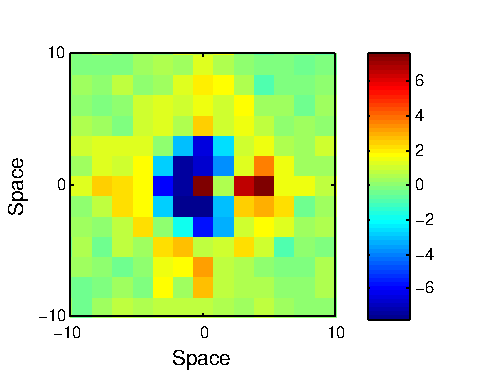
\includegraphics[scale=1]{KernelEstimateFullLinearizedPBCAniso}}
		\subfigure[]{\includegraphics[scale=1]{KernelCrossSectionLinearizedPBCAniso}}
	\caption{Linearized model to generate data. Linear model for estimation. Periodic boundary conditions.}
	\label{fig:label}
\end{figure}

\subsection{Nonlinear Neural Field Model}
\begin{figure}[htbp]
	\centering
		\subfigure[]{\includegraphics[scale=1]{KernelEstimateFullNonlinearAniso}}
		\subfigure[]{\includegraphics[scale=1]{KernelCrossSectionNonlinearAniso}}
	\caption{Nonlinear model to generate data. Linearized model for estimation. Zero boundary conditions.}
	\label{fig:label}
\end{figure}

\begin{figure}[htbp]
	\centering
		\subfigure[]{\includegraphics[scale=1]{KernelEstimateFullNonlinearPBCAniso}}
		\subfigure[]{\includegraphics[scale=1]{KernelCrossSectionNonlinearPBCAniso}}
	\caption{Nonlinear model to generate data. Linearized model for estimation. Periodic boundary conditions.}
	\label{fig:label}
\end{figure}
% \begin{figure}
% 	\centering
% 	\subfigure[]{
% 	\includegraphics[scale=1]{FieldSpatialFreq}
% 	\label{fig:ObservationSpatialFreq}}
% 	\subfigure[]{
% 	\includegraphics[scale=1]{FieldSpatialFreqCrossSection}
% 	\label{fig:ObservationSpatialFreqCrossSection}}
% 	\caption{a) Field spatial frequency in dB. b) Spatial frequency cross-section showing cutoff frequency. The black line shows the spatial frequency in the x direction and the red line shows the frequency in the y direction.}
% \end{figure}
% 
% \newpage
% 
% \begin{figure*}
% 	\centering
% 		\subfigure[]{
% 		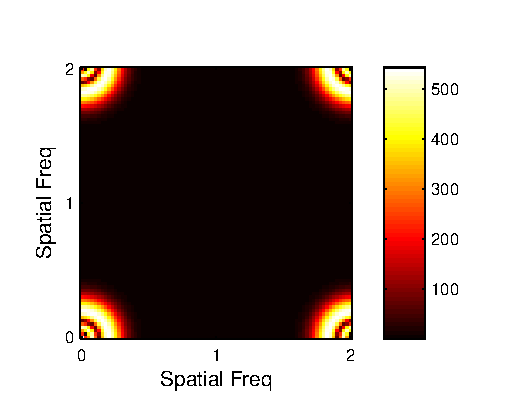
\includegraphics[scale=1]{FFTKernel}
% 	\label{fig:FFTKernel}}
% 		\subfigure[]{
% 		\includegraphics[scale=1]{FFTKernelEstimateFullLinear}
% 	\label{fig:FFTKernelEstimateFullLinear}}
% 		\subfigure[]{
% 		\includegraphics[scale=1]{FFTKernelEstimateThresholdLinear}
% 	\label{fig:FFTKernelEstimateThreshLinear}}
% 		\subfigure[]{
% 		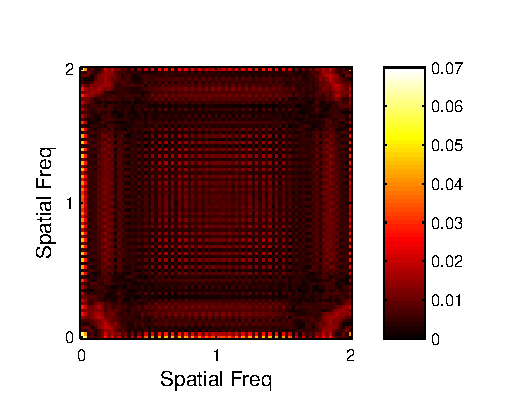
\includegraphics[scale=1]{FFTKernelEstimateFull}
% 	\label{fig:FFTKernelEstimateFullNonlinear}}
% 		\subfigure[]{
% 		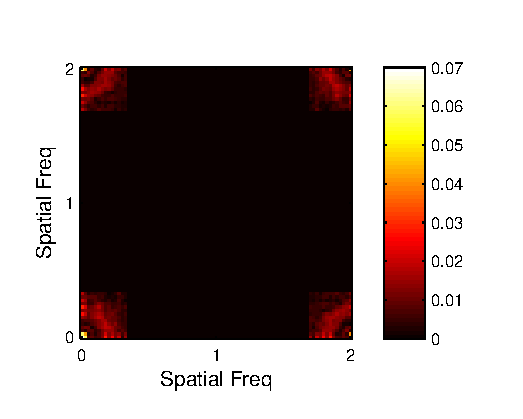
\includegraphics[scale=1]{FFTKernelEstimateThreshold}
% 	\label{fig:FFTKernelEstimateThreshNonlinear}}
% 	\label{fig:FFTKernels}
% 	\caption{a) FFT of kernel. b) FFT of kernel estimate when generating data with linear model showing numerical issues. c) Thresholded FFT of kernel estimate when generating data with linear model. d) FFT of kernel estimate when generating data with nonlinear model. e) Thresholded FFT of kernel estimate when generating data with nonlinear linear model.}
% \end{figure*}
% 
% \newpage
% 
% \begin{figure}[t!]
% 	\centering
% 		\subfigure[]{
% 		\includegraphics[scale=1]{Kernel}
% 	\label{fig:Kernel}}
% 		\subfigure[]{
% 		\includegraphics[scale=1]{KernelEstimateLinear}
% 	\label{fig:KernelEstimateLinear}}
% 		\subfigure[]{
% 		\includegraphics[scale=1]{KernelEstimate}
% 	\label{fig:KernelEstimateNonlinear}}
% 	\label{fig:Kernels}
% 	\caption{a) The actual kernel. b) Estimate of kernel when generating data using the linear model. b) Estimate of the kernel when using the nonlinear model.}
% \end{figure}
% 
% \newpage
% 
% \begin{figure}[t!]
% 	\centering
% 	\subfigure[]{
% 	\includegraphics[scale=1]{KernelsCrossSectionLinear}
% 	\label{fig:KernelCrossSectionLinear}}
% 	\subfigure[]{
% 	\includegraphics[scale=1]{KernelsCrossSection}
% 	\label{fig:KernelCrossSectionNonlinear}}
% 	\caption{a) From the linear model. b) from the nonlinear model.}
% \end{figure}
% 
% \begin{figure}[t!]
% 	\centering
% 	\subfigure[]{
% 	\includegraphics[scale=1]{FFTRemovedKernelEstimateThreshold}
% 	\label{fig:SpectrumOfEstimateWithoutKernel}}
% 	\subfigure[]{
% 	\includegraphics[scale=1]{KernelEstimateLeftOvers}
% 	\label{fig:KernelLeftOvers}}
% 	\subfigure[]{
% 	\includegraphics[scale=1]{LeftOverFromEstimate}
% 	\label{fig:KernelLeftOversCrossSection}}
% 	\caption{This part is for debugging. a) Removing the kernel from the spectrum of the estimate. b) Kernel left overs. c) Cross section of b.}
% \end{figure}
% \begin{figure}[t!]
% 	\centering
% 	\subfigure[]{
% 	\includegraphics[scale=1]{KernelEstimateParham}
% 	\label{fig:ParhamKernelCrossSectionLinear}}
% 	\caption {From the nonlinear model. left: Normalised true kernel; right: Normalised estimated kernel}
% \end{figure}
% \begin{figure}[t!]
% 	\centering
% 	\subfigure[]{
% 	\includegraphics[scale=1]{KernelsCrossSectionParham}
% 	\label{fig:ParhamKernelCrossSectionLinear}}
% 	\caption{Normalised kernel from the nonlinear model. (Black:true; Red:estimate)}
% \end{figure}

% \begin{figure}[t!]
% 	\centering
% 		\subfigure[]{
% 		\includegraphics[scale=1]{KernelEstimateDataLinsolve}
% 	\label{fig:Kernel}}
% 		\subfigure[]{
% 		\includegraphics[scale=1]{KernelEstimateDataInvConvMat}
% 	\label{fig:KernelEstimate}}
% 		\subfigure[]{
% 		\includegraphics[scale=1]{KernelEstimateDataFFT}
% 	\label{fig:KernelEstimate}}
% 	\label{fig:Kernels}
% 	\caption{Kernel estimates from data. a) Using linsolv. b) Using psuedo inverse of convolution matrix. b) Using FFT.}
% \end{figure}


\section{Discussion}

 


\section{Conclusion}
\subsection{The conclusion goes here.}




% conference papers do not normally have an appendix
\appendix
\section*{\parham{Convolution and Correlation}}
To show 
\begin{equation}
 \left(a \ast b \right)\left(\tau\right)  \star c\left(\tau\right)  = a\left(-\tau\right)\ast\left(b \star c\right)\left(\tau\right),
\end{equation}
we note that cross-correlation function is related to the convolution by \cite{Yarlagadda2009}
\begin{equation}
 \left(a \star b\right)\left(\tau\right)= a\left(-\tau \right)\ast b\left(\tau\right).
\end{equation}
Therefore, we can write
\begin{align}
 \left(a \ast b\right)\left(\tau\right) \star c\left(\tau\right)&= \left(a \ast b\right)\left(-\tau \right)\ast c\left(\tau\right) \nonumber \\
&=a\left(-\tau\right)\ast \left(b\left(-\tau\right) \ast c\left(\tau\right)\right)\nonumber \\
&=a\left(-\tau\right)\ast\left(b\star c\right)\left(\tau\right)
\end{align}



% use section* for acknowledgement
\section*{Acknowledgment}


The authors would like to thank...





\bibliographystyle{IEEEtran}
% argument is your BibTeX string definitions and bibliography database(s)
\bibliography{IEEEabrv,EMBC}


% that's all folks
\end{document}


